\documentclass[10pt,twocolumn,letterpaper]{article}

\usepackage{cvpr}
\usepackage{times}
\usepackage{epsfig}
\usepackage{graphicx}
\usepackage{amsmath}
\usepackage{amssymb}
\usepackage[utf8]{inputenc}
\usepackage{enumerate}
\usepackage{cprotect}

% Include other packages here, before hyperref.

% If you comment hyperref and then uncomment it, you should delete
% egpaper.aux before re-running latex.  (Or just hit 'q' on the first latex
% run, let it finish, and you should be clear).
\usepackage[pagebackref=true,breaklinks=true,letterpaper=true,colorlinks,bookmarks=false]{hyperref}


\cvprfinalcopy % *** Uncomment this line for the final submission

\def\cvprPaperID{****} % *** Enter the CVPR Paper ID here
\def\httilde{\mbox{\tt\raisebox{-.5ex}{\symbol{126}}}}

% Pages are numbered in submission mode, and unnumbered in camera-ready
\ifcvprfinal\pagestyle{empty}\fi

% new command for short vertical space
\newcommand{\vertbreak}{\vspace{0.5 mm}}


\begin{document}

%%%%%%%%% TITLE
\title{Semi-Supervised Learning for Text Classification}

\author{António Rodrigues\\
Faculdade de Engenharia da Universidade do Porto\\
Rua Dr. Roberto Frias S\slash N, 4200-465 Porto, Portugal\\
{\tt\small up200400437@fe.up.pt}
}

\maketitle
% \thispagestyle{empty}

%%%%%%%%% ABSTRACT
\begin{abstract}
The work presented in this paper explores the field of semi-supervised learning, 
applied to a particular problem: text classification. We explore 
a generative model for text classification --- Multinomial Naive Bayes (MNB) --- and from 
there we advance to a semi-supervised setting by combining it with the 
Expected Maximization (EM) algorithm, studying some techniques 
to augment it. We finally present results from our own and third-party 
implementations of such models, by using the well-known 20 Newsgroups dataset.
\end{abstract}


%%%%%%%%% BODY TEXT

\section{Introduction}
\label{sec:intro}

Semi-supervised learning (SSL) is a branch of machine learning that makes use of 
unlabeled data in an attempt to improve the performance of purely supervised 
learning methods in cases where labeled data is `hard to get' and scarce, when compared to 
unlabeled data~\cite{chapelle2010semi,zhu05survey,zhu2009introduction}. Such scenarios are 
rather frequent, e.g. in application areas such as text classification, image 
recognition, web content analysis. Here we focus on 
the study of specific semi-supervised classification tasks, even though other 
sub-fields such as semi-supervised regression~\cite{chapelle2010semi} 
exist.\vertbreak

The work presented in this paper explores the field of semi-supervised learning, 
applied to a particular problem: text classification. We start by exploring 
a generative model for text classification --- Multinomial Naive Bayes (MNB)~\cite{McCallum98acomparison} --- still 
in its fully-supervised form. Based on that model, we then advance to a 
semi-supervised setting by combining it with the Expected Maximization (EM)~\cite{Nigam2000} 
algorithm, studying some techniques to augment it. We finally present results 
from our own and third-party implementations of such models, over the 
well-known 20 Newsgroups dataset~\cite{Lang95}.


\section{Semi-Supervised Learning}
\label{subsec:semi-supervised}

%We now provide a brief and informal description of the main rationale behind SSL classification and 
%then develop on a particular class of methods --- Generative Models --- 
%the basis of the text classification models studied in this paper.\vertbreak

In purely Supervised Learning problems, one is given a labeled set of observations $\textbf{X}_\ell = \{\textbf{x}_1, \textbf{x}_2, ..., \textbf{x}_{|\textbf{X}_\ell|}\}$~\footnote{We will henceforth use the notation $|S|$ to represent the size of a given set $S$.} together with their class correspondences 
$\text{Y} = \{y_1, y_2, ..., y_{|\text{Y}|}\}$, taken from the joint distribution $P(\textbf{X}, \text{Y})$. The goal is to 
find a function that maps any given observation to a class, $\textbf{x} \rightarrow y_i \in \text{Y}$, such that 
the classification error is minimized.\vertbreak

Considering an SSL setting, the classification 
problem is similar --- a labeled set $\textbf{X}_\ell$ is also given, the goal is to estimate a 
relation $\textbf{x} \rightarrow y_i \in \text{Y}$ --- but now with the addition of an 
unlabeled set $\textbf{X}_u = \{\textbf{x}'_1, \textbf{x}'_2, ..., \textbf{x}'_{|\textbf{X}_u|}\}$ (i.e. without class label correspondences), where 
usually $|\textbf{X}_u| \gg |\textbf{X}_\ell|$, with samples now taken from 
the marginal distribution $P(\textbf{X})$. Starting with assumptions about the 
distribution of the data $P(\textbf{X})$ (e.g. treating it as a mixture distribution), SSL methods tackle the problem 
by supplying $\textbf{X}_u$ to unsupervised learning techniques, in order to 
reach good estimates of `hidden' (also referred to as `latent') class-conditional probabilities 
$P(\textbf{X}|\text{Z})$. The difference is that 
now the number and type of cases for Z are pre-determined by the 
class correspondences of the labeled dataset, $\text{Y}$. The assignment of 
each `latent' component of the distribution to elements in $\text{Y}$ can then be guided with 
the help of the labeled dataset, $\textbf{X}_\ell$.\vertbreak 

The success of 
SSL techniques is heavily dependent on the model's 
assumptions about the distribution of $P(\textbf{X})$, with severe negative impact on 
performance in the case of inappropriate model-to-problem 
matchings~\cite{zhu2009introduction,zhu05survey}. 
Chapelle et al.~\cite{chapelle2010semi} list the key types of assumptions often 
made by SSL methods:

\begin{itemize}

    \item \textbf{Smoothness:} If two points $x_1$ and $x_2$ are close to each other in 
            a high density region, then so should be the respective labels 
            $y_1$ and $y_2$, i.e. the labeling function is assumed to be 
            \textit{smoother} in high density regions.
    \item \textbf{Clustering or low density separation:} Points belonging to the same cluster are likely 
            to belong to the same class. Following a somewhat complementing idea to 
            `smoothness', decision boundaries should 
            lie in low-density regions.
    \item \textbf{Manifold structures}~\cite{chapelle2010semi}
    \item \textbf{Transduction}~\cite{chapelle2010semi}

\end{itemize}

% it would be great to post the assumptions in front of the methods or special 
% cases of the method classes
Several classes of SSL methods exist, each considering specialized cases of one 
(or more) of the 
aforementioned assumptions: Self-Training, Co-Training~\cite{zhu05survey}, Generative Models,
Low-Density Separation methods, Graph-Based Methods~\cite{chapelle2010semi}, among 
others~\cite{zhu05survey}.

\subsection{Semi-Supervised Generative Models}
\label{subsec:gen-models}

In their way to estimate 
$P(\text{Y}|\textbf{X})$, Generative Models (GMs) first find a $y_i \rightarrow \textbf{x}$ mapping by modeling the 
class-conditional distributions $P(\textbf{X}|\text{Y})$, instead of directly going for 
an estimation of the posteriors. In other words, GMs go through the `trouble' of 
estimating how data is generated by each element in Y 
in order to classify an observation.\vertbreak 

GMs treat $P(\textbf{X}|\text{Y})$ as 
a mixture model, where components belong to a 
family of parametric distributions (e.g. Gaussian, Multinomial, etc.), governed 
by a set of parameters 
$\theta = \{\theta_1, \theta_2, ..., \theta_n\}$. Unsupervised learning methods 
are applied over the unlabeled data $\textbf{X}_u$ in order to find estimates 
for those parameters, $\hat{\theta}$~\footnote{We represent estimations of a variable $x$ by 
topping it with an ` $\hat{}$ ' sign, $\hat{x}$.}, and identify the 
components of the mixture model, usually with a 1:1 correspondence between 
the `latent' clusters and each class in Y (Nigam et al.~\cite{Nigam2000} 
propose both 1:1 and N:1 correspondence alternatives, Zhu~\cite{zhu05survey} also points 
out that such assumptions should be carefully considered in order not to 
incur in model incorrectness). The posterior 
probabilities $P(\text{Y} = y_i|\textbf{X} = \textbf{x}, \hat{\theta})$ can then be determined via Bayes' Rule:
\[P(y_i|\textbf{x}, \hat{\theta}) = \frac{P(y_i|\hat{\theta})P(\textbf{x}|y_i,\hat{\theta})}{\sum_{i=1}^{|\text{Y}|}P(y_i|\hat{\theta})P(y_i|\textbf{x},\hat{\theta})}\]

The training of a classifier consists in 
determining the parameter estimates that maximize the likelihood 
(Maximum Likelihood estimation) of both 
labeled and unlabeled data: 
\begin{equation}
    \prod_{\textbf{x}_i \in \textbf{X}_\ell}P(y_i)P(\textbf{x}_i|y_i,\theta) \times \prod_{\textbf{x}_i \in \textbf{X}_u}\sum_{k=1}^{|\text{Y}|}P(y_k)P(\textbf{x}_i|y_k,\theta)
    \label{eq:mle}
\end{equation}

or via Maximum a Posteriori (MAP) estimation of 
$P(\theta|\textbf{X}_\ell,\textbf{X}_u)$. These estimates are usually tackled 
via gradient descent methods~\cite{chapelle2010semi} or using Expectation Maximization (EM) 
algorithms~\cite{Nigam2000}, as with the case described in Section~\ref{subsec:semi-super-em}.




\section{Methodology}
\label{sec:methodology}

The work presented here follows the consulted background literature about 
supervised and semi-supervised text classification~\cite{McCallum98acomparison,Nigam2000,Rennie03tacklingthe}, 
reflecting our understanding of the material.
%reflecting our understanding of the material.\vertbreak

%We start by introducing some of the notation used in the rest of the paper, and 
%then continue with the description of a fully supervised generative model for 
%text classification --- Multinomial Naive Bayes --- followed by semi-supervised 
%extensions to that model, which use the Expectation Maximization (EM) algorithm.

\subsection{Notation}

Text classification mainly deals with categorizing a set of text articles into 
some topic, according to a set of features such as the words contained in them. 
Here we present the notation to formalize these concepts.\vertbreak

An article $a$, 
belonging to a topic (i.e. a label\slash class) $t$, is represented by an 
array $a = \{w_{1}, w_{2}, ..., w_{|\mathcal{D}|}, t\}$, i.e. a list of 
$|\mathcal{D}|$ features and its label. In this case, each feature typically 
corresponds to the number of occurrences of the word $w_{i}$, the $i$-th word in a 
dictionary $\mathcal{D}$, within an article $a_i$. Other options for 
representing word frequency exist, such as Term Frequency and 
Inverse Document Frequency (TF-IDF)~\cite{Rennie03tacklingthe}.\vertbreak

As an example, consider an article set composed by two instances, 
$\mathcal{A} = \{a_1, a_2\}$, each one of them with the following contents:
\[a_1 : \verb+You like potato, I like potato.+\]
\[a_2 : \verb+I say tomato, you say tomato.+\]
In this case, the dictionary $\mathcal{D}$ would contain the following 
words~\footnote{As we will see in Section~\ref{subsec:exp-setup}, in practice, the 
words in $\mathcal{D}$ might be converted to a common format, e.g. all words 
converted to lowercase, stripped of punctuation, etc.}:
\[\mathcal{D} = \{\verb+You+, \verb+like+, \verb+potato+, \verb+I+, \verb+say+, \verb+tomato+\}\]
The articles $a_1$ and $a_2$ could then be codified (using the sparse 
`bag-of-words' approach~\cite{Su2011}) as:
\[a_1 = \{1, 2, 2, 1, 0, 0\}\]
\[a_2 = \{1, 0, 0, 1, 2, 2\}\]

\subsection{Generative Models for Text Classification}
\label{subsec:gen-models}

McCallum et al.~\cite{McCallum98acomparison} present two 
generative models for text classification, (1) a Multivariate Bernoulli event 
model and (2) a Multinomial event model: the first case considers multivariate 
Bernoulli as the parametric distributions describing each mixture component, 
only capturing the (non-)\,occurrence of word events in articles, while the 
second case considers Multinomial distributions, now capturing the quantity of 
word events. The authors state that the multinomial event model generally 
outperforms the multivariate Bernoulli model, specially when considering 
large dictionary sizes~\cite{McCallum98acomparison}. For the remainder of 
this paper, we focus our attention on the Multinomial event model.\vertbreak

Despite our focus on the Multinomial model, being GMs, both models assume (1) that an article $a$ is generated 
according to a mixture model, encompassing several mixture components $c_j \in 
\mathcal{C} = \{c_1, c_2, ..., c_{|\mathcal{C}|}\}$. The shape of each component 
distribution is governed by a set of parameters $\theta$. It is also assumed (2) there is a 1:1 
correspondence between the components in $\mathcal{C}$ and topics of articles 
$t_i$.\vertbreak

One can look at the process of 
`generating' an article $a_i$ in the following manner: (1) Selecting a 
component $c_j$ from the mixture model, with probability $P(c_j|\theta)$; (2) 
letting $c_j$ generate $a_i$ according to its own distribution 
$P(a_i|c_j,\theta)$. This results in the probability of an article $a_i$ being 
generated by a component $c_j$:
\begin{equation}
    P(c_j|\theta)P(a_i|c_j,\theta)
    \label{eq:data-component}
\end{equation}

As different components in $\mathcal{C}$ can contribute to origin a similar 
article $a_i$, the probability of finding an article $a_i$ is obtained by 
marginalizing expression~\ref{eq:data-component} over all the components in 
$\mathcal{C}$:
\begin{equation}
    P(a_i|\theta) = \sum_{j=1}^{|\mathcal{C}|}P(c_j|\theta)P(a_i|c_j,\theta)
    \label{eq:data-mixture}
\end{equation}

\subsection{Multinomial Naive Bayes}
\label{subsec:multinomial-naive}

The Multinomial Naive Bayes (MNB) model described by McCallum et al. 
in~\cite{McCallum98acomparison} captures the frequency of words in articles and 
applies a `bag-of-words' approach for article representation.\vertbreak 

The second step in the process of generating an article $a_i$ --- related to the 
$P(a_i|c_j,\theta)$ term in expression~\ref{eq:data-component} --- can be further 
expressed as a sequence of $|a_i|$ draws (with replacement) of words $w_k$ from 
the dictionary $\mathcal{D}$. Besides the assumptions mentioned in 
Section~\ref{subsec:gen-models}, the MNB model considers 
that (1) the length of an article $|a_i|$ (word count) is independent of the 
topic\slash mixture model component $c_j$; and (2) the appearances of words in 
an article are conditionally independent from each other, given an article 
topic: the so-called `Naive Bayes' assumption. The class conditional 
probability of an article $a_i$ can then be thought 
of as a multinomial distribution over words, with $a_i$ independent trials, in 
the form:
\begin{equation}
\begin{split}
    P(a_i|c_j,\theta) &= |a_i|!\prod_{k=1}^{|\mathcal{D}|}\frac{P(w_{k}|c_j,\theta)^{N_{i,k}}}{N_{i,k}!}\\
                &\propto \prod_{k=1}^{|\mathcal{D}|}P(w_{k}|c_j,\theta)^{N_{i,k}}
    \label{eq:data-naive}
\end{split}
\end{equation}

where $N_{i,k}$ is the number of times word $w_k$ of a dictionary $\mathcal{D}$ 
appears in an article $a_i$. In practice, as the multinomial coefficient 
$\frac{|a_i|!}{N_{i,1}! ... N_{i,|\mathcal{D}|}!}$ does not depend on the 
mixture components $c_j$, it is often ignored when the purpose is to maximize 
the likelihood $P(a_i|c_j,\theta)$~\cite{Nigam2000, Kibriya:2004:MNB:2146834.2146882, Su2011}.\vertbreak

The set of mixture model parameters $\theta$ to be estimated 
during the training phase of the classifier consists of (1) each of the class 
conditional probabilities of words 
$\hat{\theta}_{w_k|c_j} \equiv P(w_k|c_j,\hat{\theta})$; and (2) the prior 
probabilities for each topic\slash mixture model 
component $\hat{\theta}_{c_j} \equiv P(c_j|\hat{\theta})$.\vertbreak 

These estimates 
are obtained by Maximum a Posteriori (MAP) estimation of the parameters, i.e. 
we find the values of $\theta$ that maximize the posterior probability 
$P(\theta|\mathcal{A})$: 
\begin{equation}
\begin{split}
    %P(\theta|\mathcal{A}) &= \sum_{j=1}^{|\mathcal{C}|}P(c_j,\theta) \times \prod_{i=1}^{|\mathcal{A}|}P(a_i|\theta)\\
    P(\theta|\mathcal{A}) &\propto P(\theta) \times P(\mathcal{A}|\theta)
    %&\propto \prod_{j=1}^{|\mathcal{C}|} \left(\theta_{c_j}^{\sigma - 1} \prod_{k=1}^{|\mathcal{D}|} \theta_{w_k|c_j}^{\sigma - 1}\right)  \times \prod_{i=1}^{|\mathcal{A}|}P(a_i|\theta)
    \label{eq:posterior-map}
\end{split}
\end{equation}

Here we follow the same representation of $P(\theta)$ used by 
Nigam et al.~\cite{Nigam2000}, a Dirichlet distribution, with $\sigma = 2$. 
The probability $P(\mathcal{A}|\theta)$ is equal to 
$\prod_{i=1}^{|\mathcal{A}|}P(a_i|\theta)$, as one assumes the article 
generation events are independent between each other, given the mixture model 
parameters $\theta$.\vertbreak

The results of the MAP 
estimation reduce to `counting problems'. 
Specifically, $\hat{\theta}_{w_k|c_j}$ is given by the ratio of appearances of 
a word $w_k$ within all articles $a_i$ belonging to a component $c_j$ vs. the 
total number of word events for $c_j$:
\begin{equation}
\begin{split}
    \hat{\theta}_{w_k|c_j} &\equiv P(w_k|c_j,\hat{\theta})\\
    &= \frac{\alpha + \sum_{i=1}^{|\mathcal{A}|}N_{i,k}P(t_i = c_j|a_i)}{\alpha|\mathcal{D}| + \sum_{s=1}^{|\mathcal{D}|}\sum_{i=1}^{|\mathcal{A}|}N_{i,s}P(t_i = c_j|a_i)}
    \label{eq:class-cond-estimate}
\end{split}
\end{equation}

where $P(c_j|a_i) \in \{0,1\}$ depending on the label of an article $a_i$
and $N_{i,k}$ is the number of occurrences of the word $w_k$ in an article 
$a_i$. Notice the inclusion of `smoothing priors' $\alpha$, used to avoid 
probabilities equal to zero in the lack of particular word events for a 
component $c_j$. In~\cite{McCallum98acomparison,Nigam2000} the authors use 
$\alpha = 1$, which is designated by Laplace smoothing.\vertbreak

The parameters $\hat{\theta}_{c_j}$ are given 
by the ratio of the articles belonging to a component $c_j$ vs. the total 
number of articles $\mathcal{A}$:
\begin{equation}
\begin{split}
    \hat{\theta}_{c_j} &\equiv P(c_j|\hat{\theta}) = \frac{\alpha + \sum_{i=1}^{|\mathcal{A}|}P(t_i = c_j|a_i)}{\alpha|\mathcal{C}| + \sum_{i=1}^{|\mathcal{A}|}P(t_i = c_j|a_i)}
    \label{eq:prior-estimate}
\end{split}
\end{equation}

% ONE SHOULD MENTION THAT THESE EXPRESSIONS FOR PARAMETER ESTIMATIONS COME FROM 
% MAP ESTIMATION, I.E. LEARNING A CLASSIFIER IS APPROACHED BY CALCULATING A MAP 
% ESTIMATE OF THE \theta PARAMETERS.

%(...) applying the chain rule of probability~\cite{}, one can extend the second 
%term of Equation~\ref{eq:data-mixture} as follows (still without taking the 
%Naive Bayes assumption into account):

%\begin{equation}
%\begin{split}
%    P(a_i|t_j,\theta) &= P(\{N(w_{1},a_i), ..., N(w_{N},a_i)\}|c_m,\theta)\\
%    &= P(\sum_{n=1}^{N}(N(w_{n},a_i)))
%    \label{eq:data-component-chain}
%\end{split}
%\end{equation}

The final expression for the posterior 
probabilities $P(c_j|a_i,\theta)$, i.e. the probability of the class given an 
article, is obtained via Bayes' Rule:
\begin{equation}
\begin{split}
    P(c_j|a_i,\hat{\theta}) &= \frac{P(c_j|\hat{\theta})P(a_i|c_j,\hat{\theta})}{P(a_i|\hat{\theta})}\\
    &\propto P(c_j|\hat{\theta})P(a_i|c_j,\hat{\theta})
    \label{eq:posterior}
\end{split}
\end{equation}

Expression~\ref{eq:posterior} can be progressively expanded by replacing each 
one of the terms by the corresponding expressions, given in equations 
\ref{eq:data-mixture},~\ref{eq:data-naive},~\ref{eq:class-cond-estimate} and~\ref{eq:prior-estimate}.\vertbreak

Despite its unrealistic 
simplifications and assumptions (data generated by mixture model; 1:1 
correspondence between mixture components and topics; conditional independence 
of word events; article length independence), Naive Bayes classifiers have 
proven to provide fair classification 
performance~\cite{McCallum98acomparison,Nigam2000}. Due to their simplicity, 
these are well suited for text classification tasks, where the 
number of features is usually large (i.e. dictionary sizes often reaching orders 
of thousands of words~\cite{McCallum98acomparison}).

\subsection{Semi-Supervised Learning via Expectation 
Maximization (EM)}
\label{subsec:semi-super-em}

The MNB text classifier described in 
Section~\ref{subsec:multinomial-naive} falls into the scope of 
supervised learning, only taking labeled data into 
account. Despite its fair performance when trained with large amounts of 
labeled data, Nigam et al.~\cite{Nigam2000} notice how it suffers when faced 
with small-sized datasets and show some advantages (regarding 
classification accuracy) of expanding such models to the semi-supervised 
learning scope, i.e. considering both labeled and 
unlabeled data.\vertbreak 

% intro paragraph is ok. now briefly explain how the overall process works, in 
% a sequence of steps.

% now, explain the EM process with more detail, starting with the formula for 
% the probability of the data given the model P(\mathcal{A}|\theta).

As with the case of the MNB classifier, the parameters $\theta$ are obtained 
by MAP estimation, i.e. maximizing expression~\ref{eq:posterior-map}. However, 
we should note that now the training dataset is composed by the labeled and 
unlabeled subsets $\mathcal{A}^{\ell}$ and $\mathcal{A}^{u}$. Following the 
Semi-Supervised GM ideas introduced in Section~\ref{subsec:gen-models}, the expression 
for $P(\mathcal{A}|\theta)$ becomes:
\begin{equation}
\begin{split}
    P(\mathcal{A}|\theta) = &\prod_{a_i \in \mathcal{A}^{u}}\sum_{j=1}^{|\mathcal{C}|}P(c_j|\theta)P(a_i|c_j,\theta)\\ 
    &\times \prod_{a_i \in \mathcal{A}^{\ell}}P(t_i = c_j|\theta)P(a_i|t_i = c_j,\theta)
    \label{eq:data-mixture-em}
\end{split}
\end{equation}

Note that for the set of labeled articles, $\mathcal{A}^{\ell}$, one 
already knows the true topic\slash mixture model component $c_j$ which 
generated each article $a_i$, hence there is not the need of referring to all 
components in $\mathcal{C}$. However, for the unlabeled set $\mathcal{A}^{u}$, 
each component $c_j$ has a contribution to the generation of each article $a_i$ 
which must be taken into account.\vertbreak

As described in~\cite{Nigam2000} (and as with the case of the MNB 
classifier), expression~\ref{eq:data-mixture-em} can be passed to logarithmic 
form, with the maximization of $P(\theta)P(\mathcal{A}|\theta)$ being 
accomplished by solving the system of partial derivatives of 
log$(P(\theta)P(\mathcal{A}|\theta))$. Here we use the same nomenclature as that 
used in~\cite{Nigam2000}, $\ell(\theta|\mathcal{A}) \equiv 
\text{log}(P(\theta)P(\mathcal{A}|\theta))$:
\begin{equation}
\begin{split}
    \ell\left(\theta|\mathcal{A}\right) &= \text{log}\left(P(\theta)\right)\\
        &+ \sum_{a_i \in \mathcal{A}^{u}}\text{log}\left(\sum_{j=1}^{|\mathcal{C}|}P(c_j|\theta)P(a_i|c_j,\theta)\right)\\ 
        &+ \sum_{a_i \in \mathcal{A}^{\ell}}\text{log}\left(P(t_i = c_j|\theta)P(a_i|t_i = c_j,\theta)\right)
    \label{eq:log}
\end{split}
\end{equation}

The log of sums over all mixture components $\mathcal{C}$ for all $a_i \in 
\mathcal{A}^{u}$ makes the problem computationally 
intractable~\cite{Nigam2000}. This is where the EM algorithm comes into play, 
providing an iterative process to obtain a MAP estimation of the parameters 
$\theta$, including the unlabeled data~\cite{Nigam2000}. We now proceed with a brief 
description of the overall MNB + EM process, without detailing the inner works 
of EM (refer to~\cite{Nigam2000} for further details):

\begin{enumerate}

\item Train a MNB classifier with the labeled dataset $\mathcal{A}^{\ell}$ only. 
        Find the estimated parameters $\hat{\theta}$ using 
        expressions~\ref{eq:class-cond-estimate} and~\ref{eq:prior-estimate}.

\item \textbf{EM's E Step:} Use the classifier governed by the current $\hat{\theta}$ parameters to 
        estimate the contribution of each mixture model component $c_j$ to the 
        generation of each article in the unlabeled dataset $\mathcal{A}^{u}$, 
        i.e. determine $P(c_j|a_i,\hat{\theta})$ $\forall$ $a_i \in \mathcal{A}^{u}$ 
        using expression~\ref{eq:posterior}.

\item \textbf{EM's M Step:} Re-estimate the $\hat{\theta}$ parameters at the light of the new 
        $P(c_j|a_i,\hat{\theta})$ for both $\mathcal{A}^{\ell}$ and $\mathcal{A}^{u}$, using 
        expressions~\ref{eq:class-cond-estimate} and~\ref{eq:prior-estimate}. 
        Note that now $P(c_j|a_i,\hat{\theta})$ varies between 0 and 1 for $\mathcal{A}^{u}$ 
        (as opposed to $P(c_j|a_i,\hat{\theta}) \in \{0,1\}$ 
        $\forall$ $a_i \in$ $\mathcal{A}^{\ell}$).

\item Evaluate $\ell(\theta|\mathcal{A})$ using 
        expression~\ref{eq:log}. If $\Delta\ell(\theta|\mathcal{A}) > T$, 
        $T$ being a convergence threshold, return 
        to step 2. Else, accept the classifier governed by the current $\hat{\theta}$ as the final solution.

\end{enumerate}

Nigam et al.~\cite{Nigam2000} note that while this simple MNB + EM combination 
performs well over datasets containing small amounts of labeled data 
vs. large amounts of unlabeled data (e.g. with differences within the 
range of 1000 vs. 10000~\cite{Nigam2000}, in the case of the 20 Newsgroups 
dataset~\cite{Lang95}), it may decrease the classification accuracy of an MNB 
classifier in the presence of large labeled datasets. As with other 
semi-supervised learning problems~\cite{zhu2009introduction}, these reductions 
in performance are due to violations of the model assumptions, previously 
stated in Sections~\ref{subsec:gen-models} 
and~\ref{subsec:multinomial-naive}.

\subsubsection{Extensions to the EM Algorithm: EM-$\lambda$}
\label{subsubsec:semi-super-em-ext}

Nigam et al.~\cite{Nigam2000} propose two extensions to the EM approach 
described in Section~\ref{subsec:semi-super-em} which attempt to cope with 
violations of some MNB model assumptions: the EM-Multiple and EM-$\lambda$ techniques. 
In the first case, the idea is to tackle violations of the 1:1 mixture 
component-to-topic correspondence assumption, allowing N:1 correspondences. The 
idea is that some topics may be separated into sub-topics (e.g. `football' and 
`cricket' in `sports'), with co-occurrences 
of words that may be better captured by multiple multinomial distributions. The 
unsupervised learning component of the problem is now detached from a particular 
number of `soft clusters', which may be now determined via cross-validation~\cite{Nigam2000}.\vertbreak

We describe the second case -- EM-$\lambda$ -- with more detail. Notice that 
when $|\mathcal{A}^{u}| \gg |\mathcal{A}^{\ell}|$, the influence of 
$\mathcal{A}^{\ell}$ in the maximization of expression~\ref{eq:log} 
is negligible, i.e. EM will be essentially be performing unsupervised 
clustering~\cite{Nigam2000}. The role of $\mathcal{A}^{\ell}$ would then 
be limited to provide the initial parameter estimates $\hat{\theta}$ and 
provide the number and topic correspondences for the `latent' variables of the 
mixture model. This may result in poor classification accuracy if the 
distribution of the data does not follow the GM's assumptions.\vertbreak

One solution is to reduce the influence of the unlabeled data in 
expression~\ref{eq:log} by a factor $\lambda$ with 
$0 \le \lambda \le 1$. The difference between EM-$\lambda$ and the method 
shown in Section~\ref{subsec:semi-super-em} is in the M-Step, with 
equations~\ref{eq:class-cond-estimate} and~\ref{eq:prior-estimate} altered to 
include the $\lambda$ factors:
\begin{equation}
\begin{split}
    \hat{\theta}_{w_k|c_j} &\equiv P(w_k|c_j,\hat{\theta})\\
    &= \frac{\alpha + \sum_{i=1}^{|\mathcal{A}|}\Lambda(i)N_{i,k}P(t_i = c_j|a_i)}{\alpha|\mathcal{D}| + \sum_{s=1}^{|\mathcal{D}|}\sum_{i=1}^{|\mathcal{A}|}N_{i,s}P(t_i = c_j|a_i)}
    \label{eq:class-cond-estimate-lambda}
\end{split}
\end{equation}

\begin{equation}
\begin{split}
    \hat{\theta}_{c_j} &\equiv P(c_j|\hat{\theta}) = \frac{\alpha + \sum_{i=1}^{|\mathcal{A}|}\Lambda(i)P(t_i = c_j|a_i)}{\alpha|\mathcal{C}| + |\mathcal{A}^{\ell}| + \lambda|\mathcal{A}^{u}|}
    \label{eq:prior-estimate-lambda}
\end{split}
\end{equation}

where the function $\Lambda(i)$ defines the $\lambda$ weighing factor to apply, 
whether the an article $a_i$ belongs to $\mathcal{A}^{\ell}$ or 
$\mathcal{A}^{u}$:

\begin{equation}
    \Lambda(i) = \left\{ 
        \begin{array}{rl}
            \lambda &\mbox{ \text{if $a_i \in \mathcal{A}^{u}$}} \\
            1 &\mbox{ \text{if $a_i \in \mathcal{A}^{\ell}$}}
        \end{array} \right.
    \label{eq:1-final}
\end{equation}

If we consider the extreme values allowed for $\lambda$, when $\lambda = 0$ 
the influence of the unlabeled data is mitigated, resulting in a MNB classifier; 
with $\lambda = 1$ the contribution of the unlabeled dataset is maximum, 
corresponding to the basic MNB + EM approach described in 
Section~\ref{subsec:semi-super-em}. In~\cite{Nigam2000}, the value of 
$\lambda$ is chosen as that which maximizes the leave-one-out cross-validation 
classification accuracy.



\section{Implementation}
\label{sec:impl}

This section provides noteworthy details on our implementation of the methods 
introduced in Section~\ref{sec:methodology}.\vertbreak

\subsection{Multinomial Naive Bayes}
\label{subsec:multinomial-naive-impl}

The computation of the class conditional probabilities $P(a_i|c_j,\theta)$ via 
expression~\ref{eq:data-naive} involves the 
multiplication of $|\mathcal{D}|$ probabilities $P(w_{k}|c_j,\theta)$. 
Considering that text classification tasks work with dictionaries 
composed by thousands of words (e.g. $\sim$\,60000 for the 20 Newsgroups 
dataset~\cite{Lang95}), the multiplication result may end up at zero due to 
floating point precision underflow. To overcome this issue, the same 
computations can be performed in the logarithmic domain, with 
expression~\ref{eq:data-naive} becoming:
\begin{equation}
\begin{split}
    \text{log}(P(a_i|c_j,\theta)) &\propto \sum_{k=1}^{|\mathcal{D}|}N_{i,k} \times \text{log}(P(w_{k}|c_j,\theta))
    \label{eq:data-naive-log}
\end{split}
\end{equation}

\subsection{Expectation Maximization (EM)}
\label{subsec:em-impl}

As we get the values of $P(c_j|a_i,\theta)$ in logarithmic form, the floating 
point underflow problem may also arise when computing the 
`log-of-sums' component in expression~\ref{eq:log}. In order to circumvent it, 
we apply the `Log-Sum-Exp' (LSE) trick, i.e. considering:

\begin{equation}
\begin{split}
    \text{log}\sum_{j=1}^{|\mathcal{C}|}P(c_j|a_i,\theta) &= \text{log}\sum_{j=1}^{|\mathcal{C}|}e^{\text{log}(P(c_j|a_i,\theta))}\\
    &= m + \text{log}\sum_{j=1}^{|\mathcal{C}|}e^{\text{log}(P(c_j|a_i,\theta)) - m}
    \label{eq:log-sum-exp}
\end{split}
\end{equation}

where $m$ is the maximum value of $\text{log}(P(c_j|a_i,\theta))$, for each 
$a_i$. In our case we also set $P(c_j|a_i,\theta) = 0$ when 
$\text{log}(P(c_j|a_i,\theta)) - m < p$, i.e. we discard the posteriors which, 
even after LSE, are still smaller than a threshold 
$e^p$, e.g. and therefore considered too small to impact the final result. We 
also use LSE after EM's E step, before applying expression~\ref{eq:class-cond-estimate} 
over $\mathcal{A}^{u}$.\vertbreak

We only run each EM's M step (see Section~\ref{sec:methodology}), over the 
unlabeled data $\mathcal{A}^{u}$, since the 
$\hat{\theta}$ values for $\mathcal{A}^{\ell}$ are previously calculated in 
step 1 and do not change over the iterations (the respective 
$P(c_j|a_i,\hat{\theta})$ values do not change during the E step, as these 
are given).


\section{Experiments}
\label{sec:experiments}

This section describes the experiments we conducted to evaluate our and third 
party implementation of the Multinomial Naive Bayes models and respective 
semi-supervised extensions described in Section~\ref{sec:methodology}.

\subsection{Experimental Setup}
\label{subsec:exp-setup}

We start with a brief description of the dataset used in our experiments, 
followed by the plan of experiments whose results are shown 
in Section~\ref{subsec:exp-res}.

\subsubsection{Dataset}
\label{subsubsec:dataset}

We work with the 20 Newsgroups dataset~\cite{Lang95}, which consists in a 
collection of approx. 19000 web forum posts, (almost) evenly separated 
across 20 different topics~\footnote{A list of topics is available in \url{http://qwone.com/~jason/20Newsgroups/}.}. 
Although separated from each other, some of the 20 classes are related to each other as sub-topics of a larger 
category (e.g. \verb+rec.sport.baseball+ and \verb+rec.sport.baseball+ as 
sub-topics of \verb+rec.sport.*+). The posts were collected over a period 
of several months in 1993~\cite{Nigam2000}.\vertbreak 

For our 
experiments, we consider a modified version of the \verb+20news-bydate+ 
dataset~\footnote{Available in \url{http://qwone.com/~jason/20Newsgroups/}.}. 
The \verb+20news-bydate+ provides a dataset 
sorted by date, with separate training and test subsets (test subset composed by later posts), comprising a total of 
18846 newsgroups articles. 
Using the Rainbow tools~\cprotect\footnote{Available in \url{http://www.cs.cmu.edu/~mccallum/bow/rainbow/}. Due to compiling issues with the original versions 
of Rainbow, we have used the following patched version which compiles 
with \verb+gcc+ version 4.6.3: \url{https://github.com/brendano/bow/}.}, developed by the authors of~\cite{McCallum98acomparison,Nigam2000}, we have 
modified the dataset to (1) remove newsgroups headers (a common practice since 
the article headers include the name of the newsgroup they belong to, which 
would make classification trivial), (2) remove 524 common `stop words' (e.g. 
`the', `of') and (3) remove words which occur only 1 time. These feature 
selection approaches are made 
in previous works on text 
classification~\cite{McCallum98acomparison,Nigam2000,Kibriya:2004:MNB:2146834.2146882,Su2011} and are mainly used as 
attempts to reduce the data dimensionality (i.e. size of the dictionary, 
$|\mathcal{D}|$. We have noticed that (2) was necessary to achieve similar MNB 
accuracies to those reported in~\cite{McCallum98acomparison,Nigam2000}. The characteristics of the modified 
\verb+20news-bydate+ are summarized in Table~\ref{tab:dataset-chars}.

\begin{table}
    \begin{center}
        \begin{tabular}{|l|c|c|}
            \hline
            \textbf{Partition}   & \textbf{\# Articles}   & \textbf{\# Unique Words} \\
            \hline\hline
            Training    & 11260         & 53485 \\
            Test        & 7502          & 60698 \\
            \hline
        \end{tabular}
    \end{center}
    \cprotect\caption{Characteristics of version of \verb+20news-bydate+ dataset used in experiments.}
    \label{tab:dataset-chars}
\end{table}

\subsubsection{Experimental Protocol}
\label{subsubsec:protocol}

The protocol is structured to test the different methods presented in 
Section~\ref{sec:methodology}, in the same order.\vertbreak

\textbf{A) Multinomial Naive Bayes}\vertbreak

We test our implementation of the MNB classifier, together with Rainbow's, 
evaluating accuracy and confusion between actual and predicted classifications 
under different conditions. We evaluate total and per-class accuracy $Acc$ in 
\%, according to expression~\ref{eq:acc}:

\begin{equation}
    Acc = \frac{\text{\# correctly classified articles}}{\text{total \# classified articles}}
    \label{eq:acc}
\end{equation}

The MNB classifiers are tested over the test set (see 
Table~\ref{tab:dataset-chars}), for different sample sizes 
$|\mathcal{A}^{\ell}| = \{20, 50, 100, 500, 1000, 5000, 7520\}$ from the training set. 
For each case, we randomly sample $|\mathcal{A}^{\ell}| / 20$ articles 
from each of the 20 topics and show the average results over 20 runs of this procedure.\vertbreak

\textbf{B) Multinomial Naive Bayes + EM}\vertbreak

We test our implementation of the MNB + EM combination, together with Rainbow's, 
again evaluating accuracy and confusion between actual and predicted classifications 
under different conditions. The selection of $\mathcal{A}^{\ell}$ and 
$\mathcal{A}^{u}$ sets is done as follows:

\begin{enumerate}

    \item We first select a $\mathcal{A}^{\ell}$ sample of size 
        $|\mathcal{A}^{\ell}| = \{20, 40, 100, 300, 500, 800, 1000, 1260\}$ from 
        the training subset, again $|\mathcal{A}^{\ell}| / 20$ articles 
        from each of the 20 topics.
    \item We use the remaining $11260 - |\mathcal{A}^{\ell}|$ as unlabeled 
        data $\mathcal{A}^{u}$.

\end{enumerate}

The values of $|\mathcal{A}^{\ell}|$ are chosen so that 
$|\mathcal{A}^{u} \ge 10000|$, for comparison with the results from~\cite{Nigam2000}. 
Again, we show the average results over 20 runs of this procedure. As a 
baseline for direct comparison we use the 
results for the fully supervised MNB classifier, trained with each different 
$\mathcal{A}^{\ell}$ set.\vertbreak

\textbf{C) Multinomial Naive Bayes + EM-$\lambda$}\vertbreak

We test our implementation of the MNB + EM-$\lambda$ combination, in a similar 
way to that of the basic EM case. Here we additionally test several values of 
$\lambda = \{0.01, 0.02, 0.1, 0.2, 0.5, 1.0\}$, evaluating accuracy and confusion 
between actual and predicted classifications.

\subsection{Experimental Results}
\label{subsec:exp-res}

We present the results for the experiments described in the previous section. 
Due to problems with our implementation of EM and 
EM-$\lambda$\,\footnote{Errors in the M-step of the EM algorithm. The code 
is available in \url{http://paginas.fe.up.pt/~up200400437/mlproject.zip} for 
reference}, we only compare 
our implementation of MNB in MATLAB to that of the Rainbow 
framework. Nevertheless, we provide the results obtained with Rainbow, using 
the modified version of the \verb+20news-bydate+ dataset.\vertbreak

In Figure~\ref{fig:mnb} we present the results of the supervised MNB 
classifier. The accuracy values for the Rainbow's version closely follow those 
reported in~\cite{Nigam2000}. For low values of $|A^\ell|$, our implementation 
of MNB (which follows the methodology provided in Section~\ref{subsec:multinomial-naive}) provides 
worse results than Rainbow's, with closer values for $|A^\ell| > 5000$.\vertbreak

\begin{figure}[h!]

    \centering
    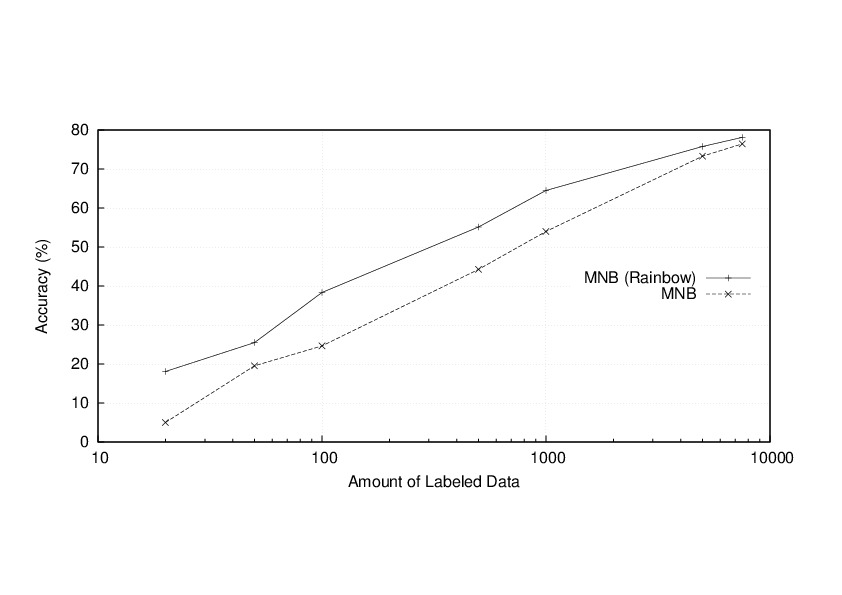
\includegraphics[width=0.40\textwidth]{figures/mnb.pdf}
    \cprotect\caption{Results for test A: MNB, using Rainbow's framework and 
        our implementation in MATLAB.}
    \label{fig:mnb}

\end{figure}

The results for test B, shown in Figure~\ref{fig:mnb-em}, partly reproduce the 
results found in~\cite{Nigam2000}, since for the lower $|A^\ell|$ the average 
results of MNB + EM surpass those for MNB. For $|A^\ell| > 40$, MNB provides 
better accuracies, nevertheless one should 
note we use a larger testing set (7502 vs. 4000) and a different method 
for choosing $A^\ell$ and $A^u$. MNB + EM accuracy strongly varies during 
the 20 runs, consistently providing higher maximums and lower minimums than 
MNB, for all $|A^\ell|$ (see Figure~\ref{fig:mnb-em-max-min}). The maximum values 
for MNB + EM approach those reported in~\cite{Nigam2000}. 
Figures~\ref{fig:mnb-em-mnb} and~\ref{fig:mnb-em-em} show four cases of 
confusion matrices for test B, $A^\ell = 1260$, for both MNB and MNB + EM 
methods. One can clearly verify EM's clustering nature on the right side of 
Figure~\ref{fig:mnb-em-max-min}, with a significant number of false predictions 
for articles belonging to \verb+comp.*+ subgroups, mostly classified as 
belonging to the class \verb+comp.graphics+. As expected, the main focus of 
confusion occur for clusters of subgroups, namely \verb+comp.*+, \verb+sci.*+ (with a considerable 
number of articles belonging to several \verb+comp.*+ subgroups being misclassified 
as \verb+sci.crypt+) and \verb+talk.*+, for both MNB and MNB + EM cases.

\begin{figure}[h!]

    \centering
    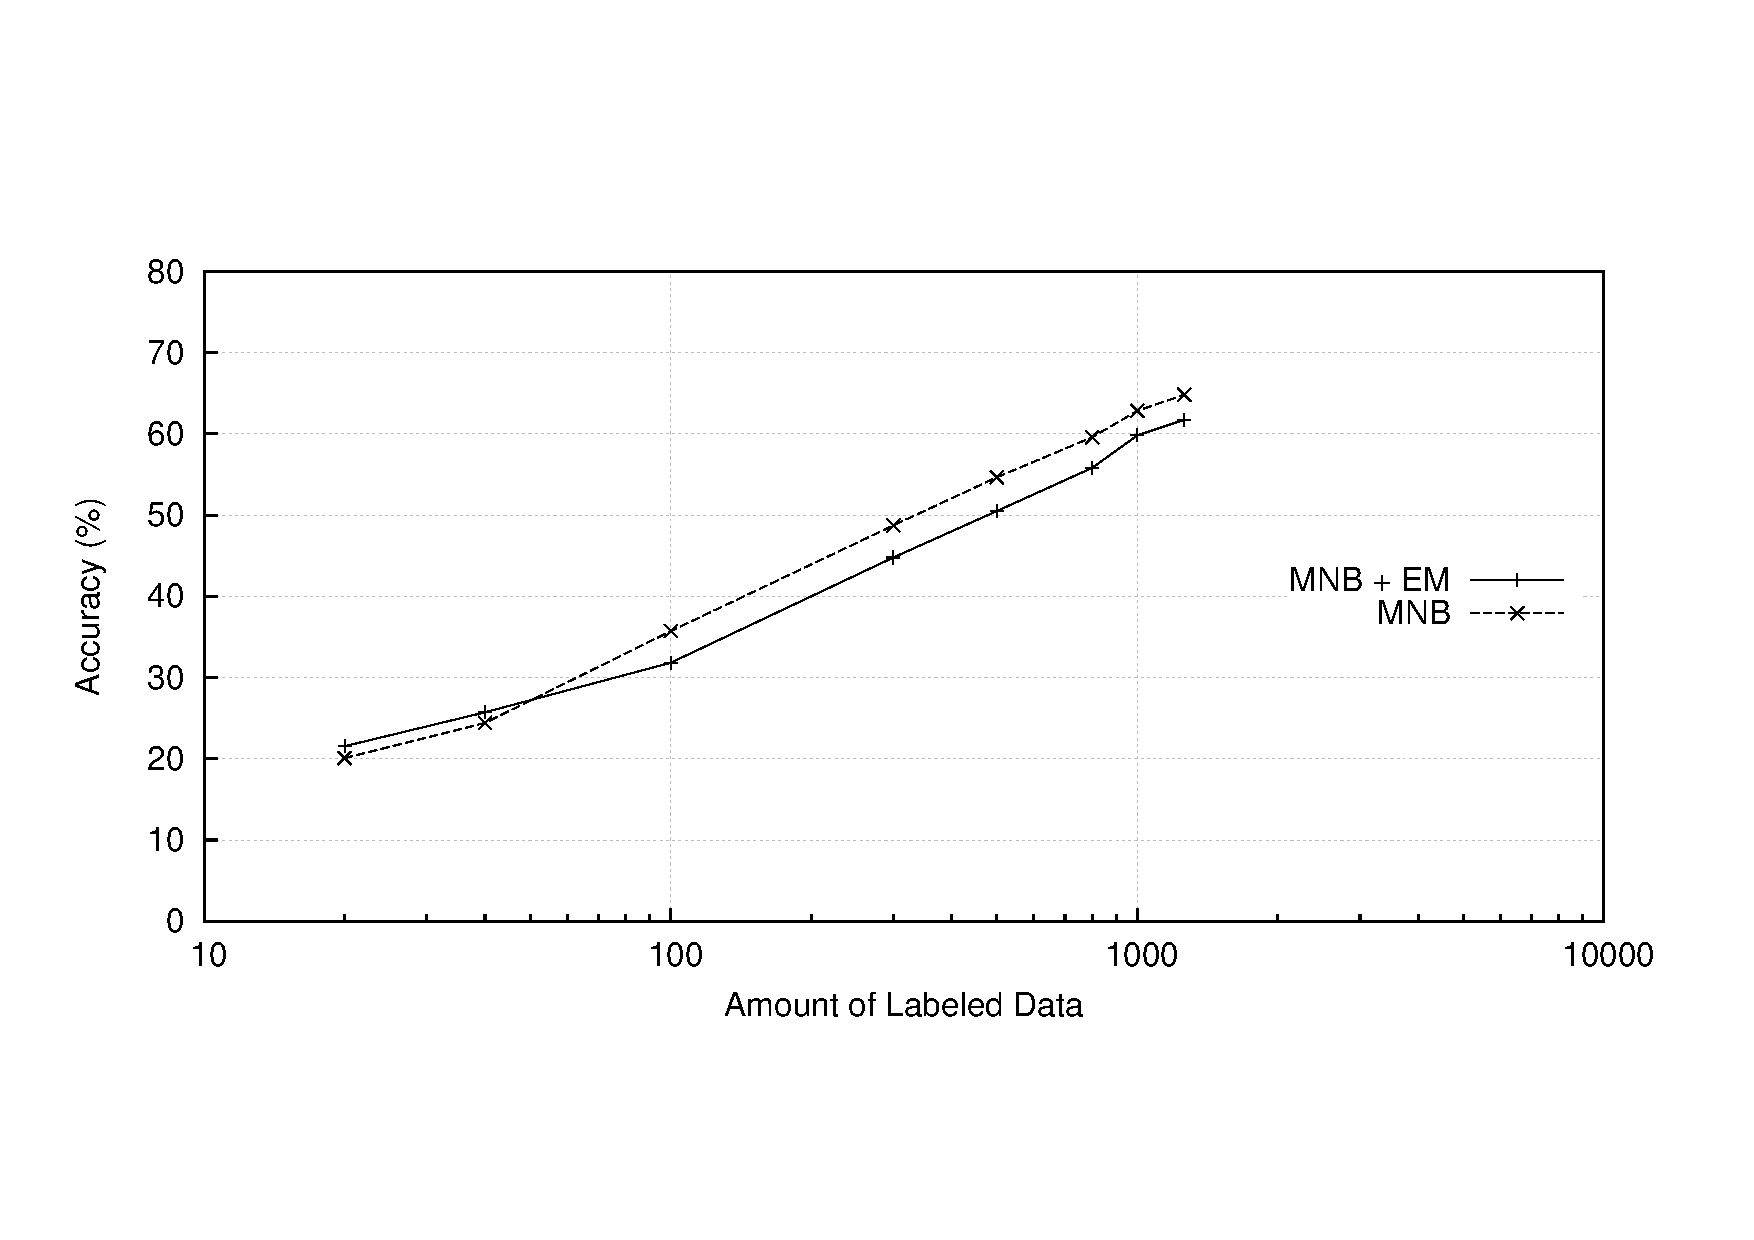
\includegraphics[width=0.40\textwidth]{figures/em.pdf}
    \cprotect\caption{Results for test B: MNB + EM, using Rainbow's framework. 
        The results of MNB for the same $A^\ell$ are also given.}
    \label{fig:mnb-em}

\end{figure}

\begin{figure}[h!]

    \centering
    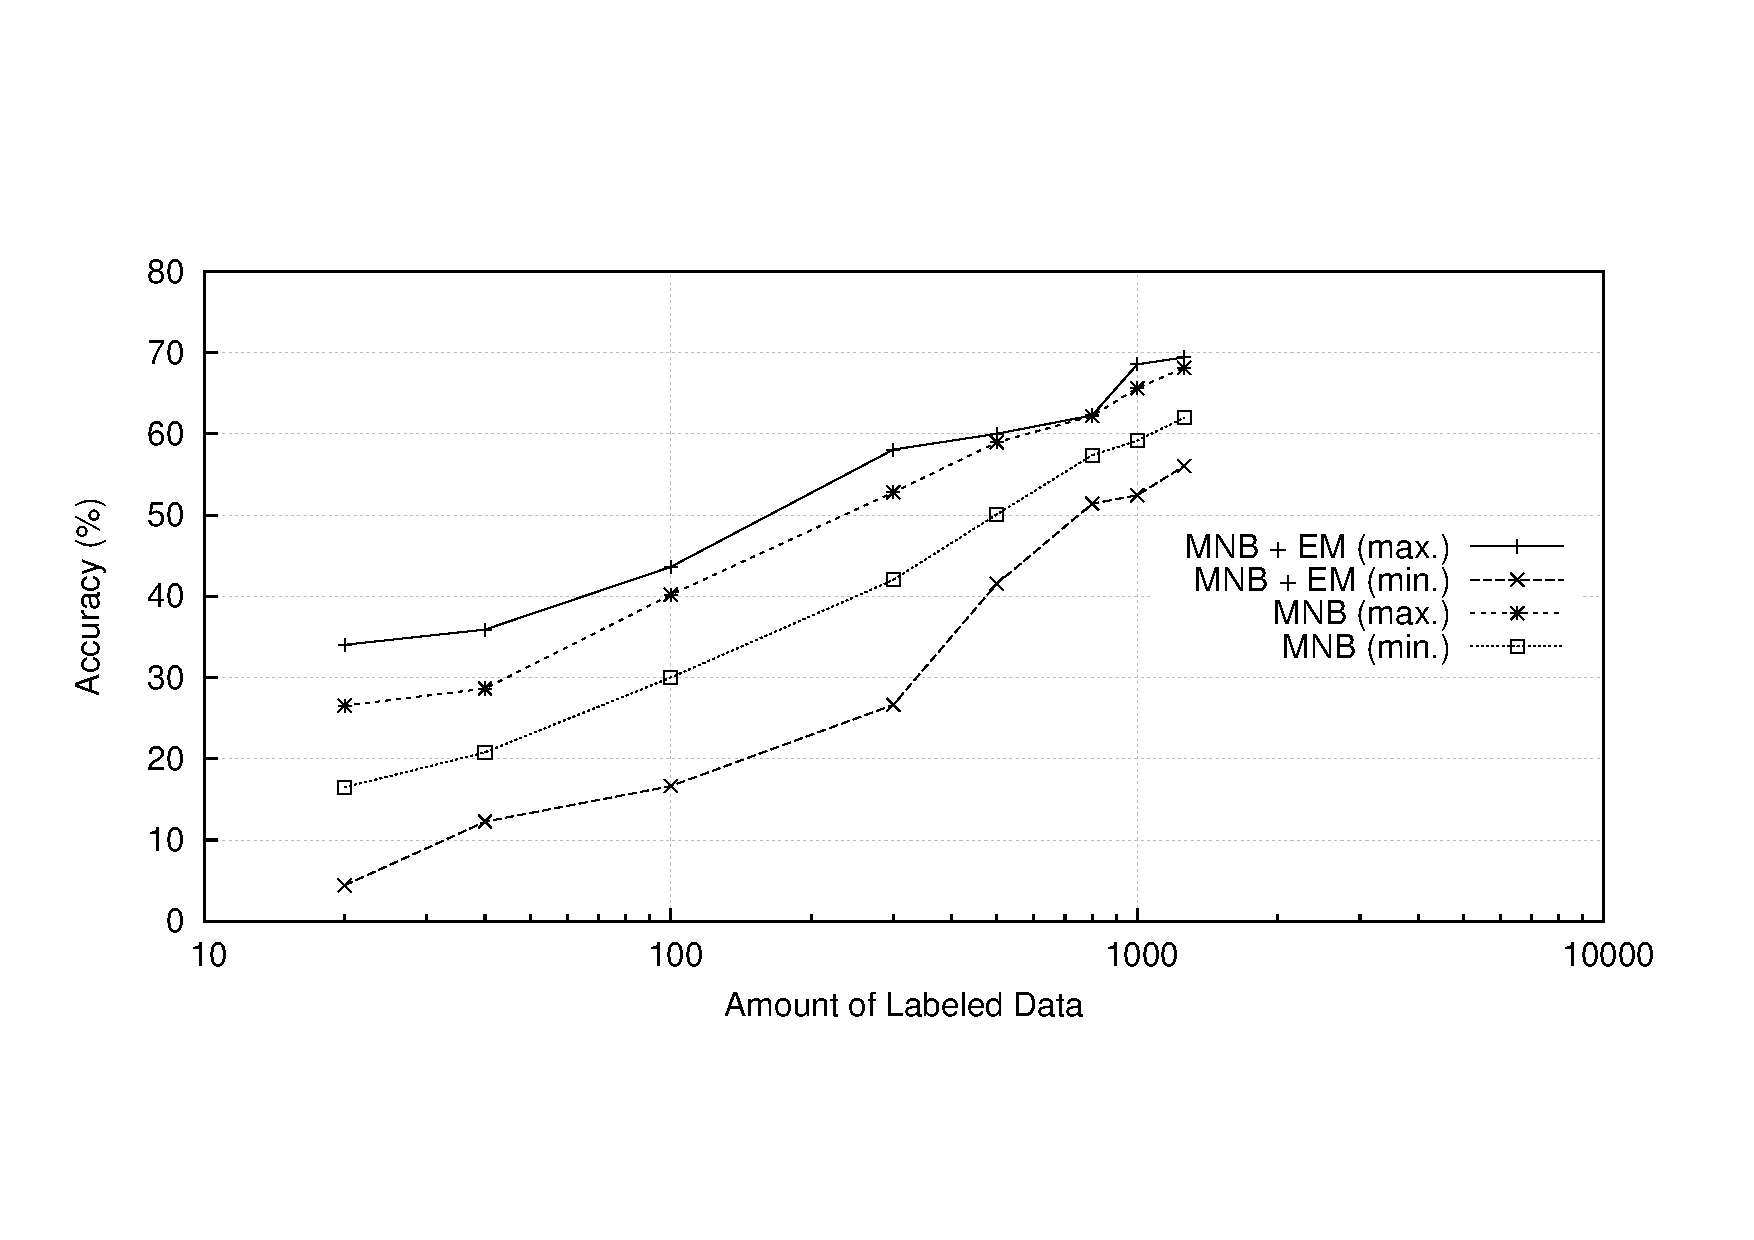
\includegraphics[width=0.40\textwidth]{figures/em-max-min.pdf}
    \cprotect\caption{Results for test B: MNB + EM, using Rainbow's framework. 
        The results of MNB for the same $A^\ell$ are also given.}
    \label{fig:mnb-em-max-min}

\end{figure}

\begin{figure}[h!]

    \centering
    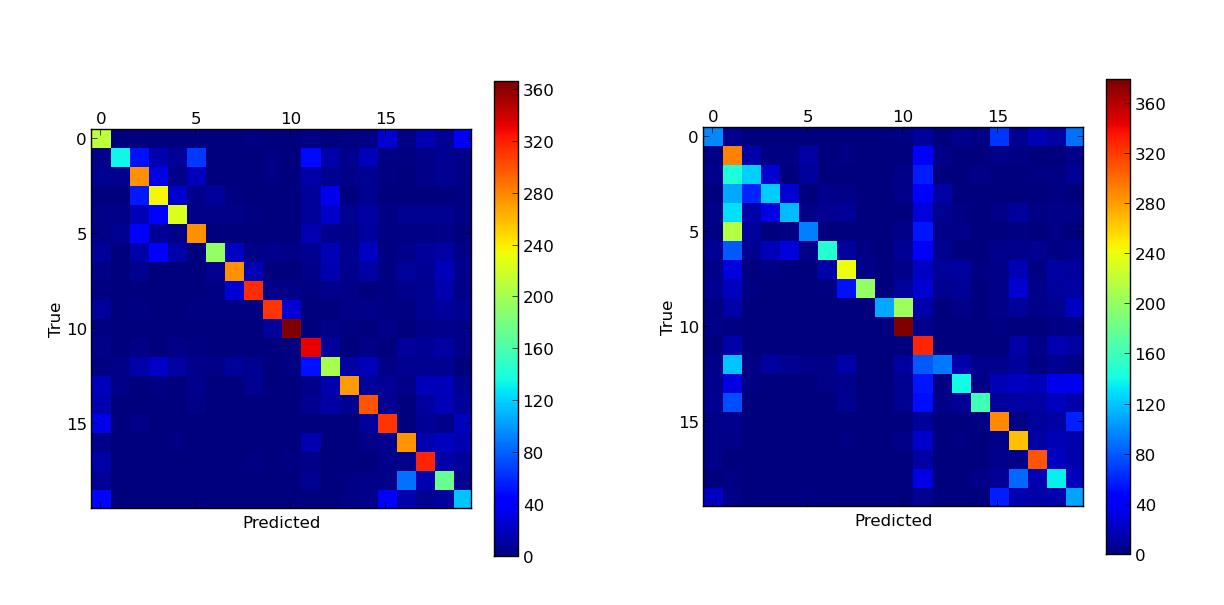
\includegraphics[width=0.45\textwidth]{figures/mnb-conf-1260.png}
    \cprotect\caption{Results for test B: Confusion matrices for best (68.12 \%) 
        and worst (61.99 \%) results of 
        MNB, $|A^\ell| = 1260$.}
    \label{fig:mnb-em-mnb}

\end{figure}

\begin{figure}[h!]

    \centering
    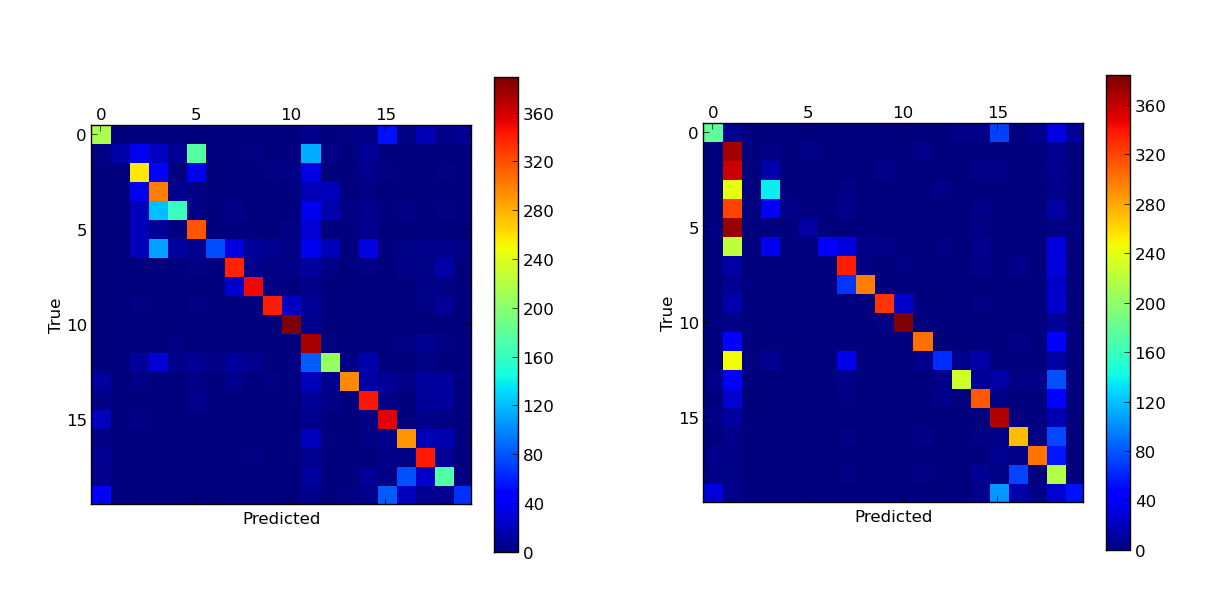
\includegraphics[width=0.45\textwidth]{figures/em-conf-1260.png}
    \cprotect\caption{Results for test B: Confusion matrices for best (left side, 69.44 \%) 
        and worst (right side, 56.04 \%) results of 
        MNB + EM, $|A^\ell| = 1260$.}
    \label{fig:mnb-em-em}

\end{figure}

Figure~\ref{fig:mnb-em-lambda} shows the results for the EM-$\lambda$ method, 
for several values of $L = 1 / \lambda$\,\cprotect\footnote{We use Rainbow's option 
\verb+--em-unlabeled-normalizer+, which determines the number of unlabeled 
articles it takes to equal a labeled article.}. We verified that for low values 
of $|A^\ell|$, lower values of $L$ (and therefore higher $\lambda$) provide 
better results, with the top accuracy verified for $\lambda = 1$. As $|A^\ell|$ 
increases, higher accuracy values tend to be favored by lower values of $\lambda$. 
Nevertheless, the best results for EM-$\lambda$ keep occurring for $\lambda = 1$, 
which seems somewhat counter-intuitive.

\begin{figure}[h!]

    \centering
    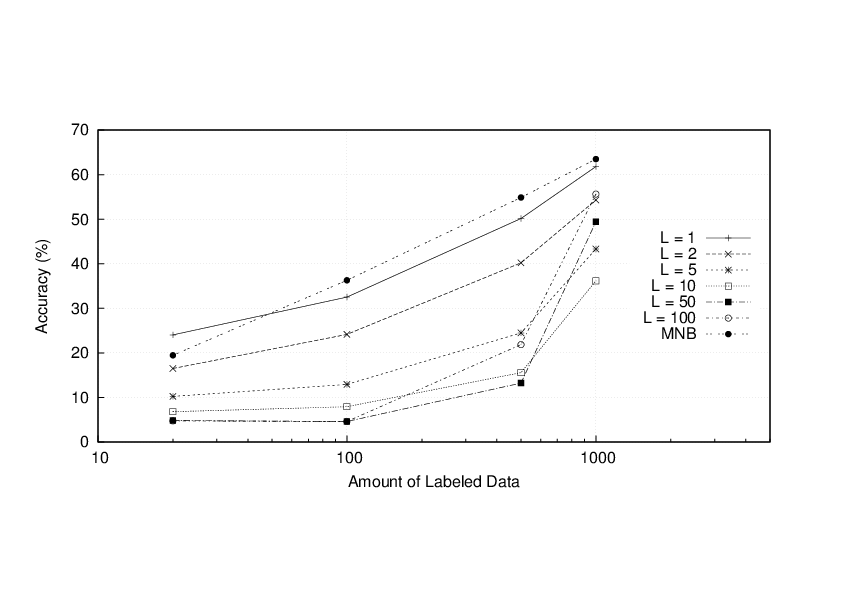
\includegraphics[width=0.40\textwidth]{figures/em-lambda.pdf}
    \cprotect\caption{Results for test C: MNB + EM-$\lambda$, using Rainbow's framework. 
        The results of MNB for the same $A^\ell$ are also given.}
    \label{fig:mnb-em-lambda}

\end{figure}


\section{Related Work}
\label{sec:rel-work}

The study of techniques for text classification presented here is mostly 
based on the work by McCallum et al.~\cite{McCallum98acomparison} and 
Nigam et al.~\cite{Nigam2000}, extensively covered 
in Section~\ref{sec:methodology}. Within the field of supervised 
learning, starting from the MNB model presented 
in~\cite{McCallum98acomparison}, Rennie et al.~\cite{Rennie03tacklingthe} 
propose a series of transforms, based on Information Retrieval 
techniques, which improve the performance of MNB, resulting 
in an enhanced method designated by Transformed Weight-normalized Complement 
Naive Bayes (TWCNB). In the semi-supervised scope, Mann et al.~\cite{Mann2007a} 
proposed a general approach to semi-supervised learning, but tested on 
text classification, designated by Expectation 
Regularization (XR)~\cite{Mann2007a}. XR is based on exponential-family 
parametric models, normally trained by MAP estimation. XR adds it with a second 
term, which attempts to minimize the difference between 
the predicted posteriors $P(Y|X)$ for unlabeled data and estimated pre-known 
values for $P(Y|X)$, obtained from empirical 
data or the labeled data. The method is tested against MNB and MNB + EM, being 
outperformed by the two in the Simulated\slash Real\slash Aviation\slash Auto 
(SRAA) text classification task, similar to 20 Newsgroups task.\vertbreak


\section{Conclusions}

In this work we study the field of semi-supervised learning, applied to the 
field of text classification. We closely follow the work in~\cite{McCallum98acomparison,Nigam2000}, reporting out 
understanding of the presented models.\vertbreak

We follow the methods presented by Nigam et al.~\cite{Nigam2000} to implement our 
versions of the MNB and MNB + EM (including EM-$\lambda$) approaches. We 
take the well-known 20 Newsgroups dataset~\cite{Lang95}, particularly 
a version designated by \verb+20news-bydate+, to evaluate the studied 
semi-supervised models in the context of a real-world dataset. The 
\verb+20news-bydate+ dataset is manipulated using the Rainbow tools --- developed 
by the authors of the base literature reviewed in this paper --- in order to 
pre-process it according to commonly used procedures and divide it 
into training and test partitions, also creating unlabeled samples for the 
semi-supervised setting.\vertbreak

Our version of MNB is compared with Rainbow's, producing lower accuracy values 
for small amounts of labeled data, approaching Rainbow's accuracy rates for 
higher amounts of labeled data ($|A^\ell| > 5000$). Due to problems with our 
implementation of MNB + EM, making its results unsuitable for comparison, we 
use Rainbow's implementation of MNB + EM and EM-$\lambda$ over the 
\verb+20news-bydate+ dataset to experimentally validate the previously studied 
semi-supervised methods. We verify that, on average MNB + EM performs better 
than MNB for $|A^\ell| < 100$, with $11220 \le |A^u| \le 11240$. We also verify that, 
despite its large variations, for at least one of the test runs performed 
for every $|A^\ell|$, MNB + EM surpasses MNB. Regarding EM-$\lambda$, while 
smaller weights for unlabeled data seem to favor accuracy for larger 
$|A^\ell|$, the best results are always obtained for $\lambda = 1$. For 
$|A^\ell| \ge 1000$, the results seem intuitive, as the accuracy approaches 
that of MNB for smaller values of $\lambda$ (i.e. smaller weights given to 
the unlabeled data).


%%%%%%%%% BODY TEXT END

{\small
\bibliographystyle{ieee}
\bibliography{egpaper_for_review}
}

\newpage
\rule{0pt}{1pt}\newpage
\rule{0pt}{1pt}\newpage
\rule{0pt}{1pt}\newpage
\rule{0pt}{1pt}\newpage
\rule{0pt}{1pt}\newpage
\rule{0pt}{1pt}\newpage
\rule{0pt}{1pt}\newpage
\rule{0pt}{1pt}\newpage

\end{document}
